\documentclass[11pt,hyperref={bookmarks=false}]{beamer}
\usetheme{Warsaw}
%\usetheme{Madrid}
%\usecolortheme{beaver}
\usefonttheme{professionalfonts}
 \usepackage[usenames,dvipsnames]{pstricks}
 \usepackage{wallpaper}
 \usepackage{epsfig}
\definecolor{UniBlue}{RGB}{157,34,53}
\setbeamercolor{block title}{bg=UniBlue!70,fg=black}

\usepackage{psfrag,graphicx}
\usepackage{amsmath,amsfonts}
\usepackage{lscape}
\usepackage{array,epsfig}
\usepackage{amsfonts}
\usepackage{amssymb}
\usepackage{amsxtra}
\usepackage{amsthm}
\usepackage{makecell}
\usepackage[skip=0pt, belowskip=-10pt]{caption}
\usepackage{subcaption}
\usepackage{float}
\usepackage{multirow}
\usepackage{booktabs}
%\usepackage{subfigure}
\usepackage{eso-pic}
\usepackage{transparent}
\usepackage{graphicx}
\usepackage{tikz}
\usepackage{longtable}
\newtheorem{df}{Definition}
\newtheorem{lm}{Lemma}
\newtheorem{prp}{Proposition}
\newtheorem{sprf}{Sketch of Proof}
\newtheorem{prf}{Proof}
\newtheorem{conjecture}{Conjecture}
\newtheorem{suffc}{Sufficient Condition}
\setbeameroption{hide notes}
\newcommand{\threelinebracer}{$\left. \begin{array}{c} \\ \\ \\ \end{array} \right\rbrace$}
\newcommand{\threelinebracel}{$\left. \begin{array}{c} \\ \\ \\ \end{array} \right\lbrace$}
\newcommand{\twolinebracer}{$\left. \begin{array}{c} \\ \\ \end{array} \right\rbrace$}
\newcommand{\twolinebracel}{$\left. \begin{array}{c} \\ \\ \end{array} \right\lbrace$}
\newcommand{\bd}{\partial}

\usepackage{pgf}  
%\logo{\pgfputat{\pgfxy(-1.2,-0.2)}{\pgfbox[center,base]{\includegraphics[height=12pt, keepaspectratio]{UA_Logo_Horizontal.eps}}} }

%\usebackgroundtemplate
%{
  %  \node[opacity=0.3, at=(current page.south east),anchor=south east,inner sep=0pt] 
    %\includegraphics[width=\paperwidth,height=20pt]{UA_Logo_Horizontal.eps}%
%}

\linespread{1}
\usepackage{parskip}
%\setlength{\itemsep}{1em} 
%\addtolength{\parskip}{5pt}
\DeclareMathSizes{12}{10}{8}{6}
%  \begin{itemize}}{\end{itemize}}
% Separate slides by \begin{frame} and \end{frame}.
\title[Willingness-to-pay for Warnings]{Willingness-to-pay for Warnings}
\author[A. Gaduh, P. McGee and A. Ugarov]{A. Gaduh, P. McGee and A. Ugarov}
\institute[]{}
\date{\today}


\begin{document}
%\AddToShipoutPicture*{\BackgroundPic}

\begin{frame}
\titlepage
\end{frame}

%%%%%%%%%%%%%%%%%%%%%%%%%%%%%%%%%%%%%%%%%%%%%%%%%%%%%%%%%%%%%%%%%%%%%%%%%%%%%%%%%%%%%%%%%%%%%%%%
%%%%%%%%%%%%%%%%%%%%%%%%%%%%%%%%%%%%%%%%%%%%%%%%%%%%%%%%%%%%%%%%%%%%%%%%%%%%%%%%%%%%%%%%%%%%%%%%



\begin{frame}
\frametitle{Motivation}
\begin{itemize}
\item Subjects underweight both the prior probability and the signal (consistent with all the tasks using signals)
\item Subjects tend to approach tasks independently
\item Subjects's WTP underreact to false positive rates for low priors and overreact for high probabilities
\item The oppositve is true for false negative rates
\item WTP is overly sensitive to false positive and false negative rates
\end{itemize}
\end{frame}



\begin{frame}
\frametitle{Research Question}
\begin{itemize}
\item Subjects underweight both the prior probability and the signal (consistent with all the tasks using signals)
\item Subjects tend to approach tasks independently
\item Subjects's WTP underreact to false positive rates for low priors and overreact for high probabilities
\item The oppositve is true for false negative rates
\item WTP is overly sensitive to false positive and false negative rates
\end{itemize}
\end{frame}



\begin{frame}
\frametitle{Summary}
\begin{itemize}
\item Subjects underweight both the prior probability and the signal (consistent with all the tasks using signals)
\item Subjects tend to approach tasks independently
\item Subjects's WTP underreact to false positive rates for low priors and overreact for high probabilities
\item The oppositve is true for false negative rates
\end{itemize}
\end{frame}


\begin{frame}
\frametitle{Model}
\begin{itemize}
\item Subjects underweight both the prior probability and the signal (consistent with all the tasks using signals)
\item Subjects tend to approach tasks independently
\item Subjects's WTP underreact to false positive rates for low priors and overreact for high probabilities
\item The opposite is true for false negative rates
\end{itemize}
\end{frame}



\begin{frame}
\frametitle{Experimental Design}
\begin{itemize}
\item Subjects underweight both the prior probability and the signal (consistent with all the tasks using signals)
\item Subjects tend to approach tasks independently
\item Subjects's WTP underreact to false positive rates for low priors and overreact for high probabilities
\item The opposite is true for false negative rates
\end{itemize}
\end{frame}



\begin{frame}
\frametitle{WTP for signals: Determinants}
\footnotesize
\begin{table}[htbp]\centering
\def\sym#1{\ifmmode^{#1}\else\(^{#1}\)\fi}
\caption{WTP for Information (Discrepancy)}
\begin{tabular}{l*{6}{c}}
\hline\hline
                &\multicolumn{1}{c}{(1)}&\multicolumn{1}{c}{(2)}&\multicolumn{1}{c}{(3)}&\multicolumn{1}{c}{(4)}&\multicolumn{1}{c}{(5)}&\multicolumn{1}{c}{(6)}\\
                &\multicolumn{1}{c}{}&\multicolumn{1}{c}{}&\multicolumn{1}{c}{}&\multicolumn{1}{c}{}&\multicolumn{1}{c}{}&\multicolumn{1}{c}{}\\
\hline
FP costs        &      .17         &     .213\sym{*}  &     .062         &    .0744         &     .338\sym{*}  &      .37\sym{**} \\
                &    (0.1)         &    (0.1)         &    (0.2)         &    (0.2)         &    (0.2)         &    (0.2)         \\
FN costs        &       .3\sym{***}&     .246\sym{***}&     .329\sym{***}&     .314\sym{***}&     .367\sym{***}&      .32\sym{***}\\
                &    (0.1)         &    (0.1)         &    (0.1)         &    (0.1)         &    (0.1)         &    (0.1)         \\
Risk-averse     &                  &                  &  -.00425         &    -.231         &                  &                  \\
                &                  &                  &    (0.3)         &    (0.4)         &                  &                  \\
Risk-averse $\times$ FP costs&                  &                  &     .145         &     .217         &                  &                  \\
                &                  &                  &    (0.2)         &    (0.2)         &                  &                  \\
Risk-averse $\times$ FN costs&                  &                  &   -.0312         &    -.125         &                  &                  \\
                &                  &                  &    (0.1)         &    (0.1)         &                  &                  \\
Accur. beliefs  &                  &                  &                  &                  &     .132         &     .221         \\
                &                  &                  &                  &                  &    (0.3)         &    (0.4)         \\
Accur. beliefs $\times$ FP costs&                  &                  &                  &                  &    -.381\sym{*}  &    -.365         \\
                &                  &                  &                  &                  &    (0.2)         &    (0.2)         \\
Accur. beliefs $\times$ FN costs&                  &                  &                  &                  &    -.133         &    -.145         \\
                &                  &                  &                  &                  &    (0.1)         &    (0.1)         \\
Constant        &    -.111         &     .413\sym{**} &    -.139         &     .463\sym{*}  &    -.173         &     .311         \\
                &    (0.1)         &    (0.2)         &    (0.2)         &    (0.3)         &    (0.2)         &    (0.3)         \\
Prior dummies   &       No         &      Yes         &       No         &      Yes         &       No         &      Yes         \\
\hline
Observations    &      744         &      744         &      690         &      690         &      744         &      744         \\
Adjusted \(R^{2}\)&     0.03         &     0.20         &     0.03         &     0.21         &     0.03         &     0.21         \\
\hline\hline
\multicolumn{7}{l}{\footnotesize Standard errors in parentheses}\\
\multicolumn{7}{l}{\footnotesize \sym{*} \(p<0.10\), \sym{**} \(p<0.05\), \sym{***} \(p<0.01\)}\\
\end{tabular}
\end{table}


\end{frame}


\begin{frame}
\frametitle{WTP Sensitivity}
\begin{figure}[h]
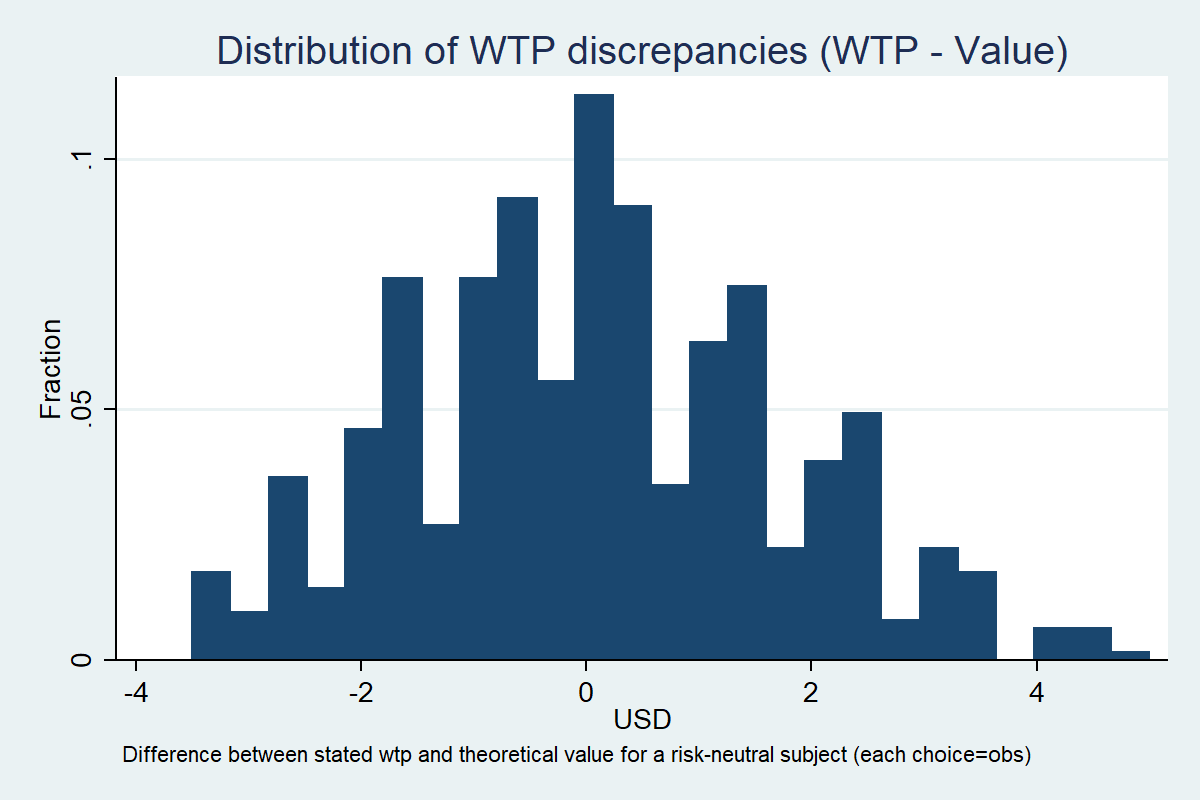
\includegraphics[scale=0.3]{Graphs/hist_WTP_discr1.png}
\end{figure}
\end{frame}


\begin{frame}
\frametitle{WTP Big Picture}
\small
\begin{table}[H]\centering \caption{Average WTP discrepancy (WTP-Value) by Signal Type} 
\label{tab:WTP_nonpar}
\begin{tabular}{cccc} \hline \hline
\textbf{False-positive}&\textbf{False-negative}&\textbf{Mean WTP discrepancy}& \textbf{P($=0$)}\\ \hline
No&No&-0.106&0.433\\
No&Yes&0.143&0.250\\
Yes&No&0.081&0.502\\
Yes&Yes&0.492&0.000\\
\hline \end{tabular} \end{table}

\end{frame}


\begin{frame}
\frametitle{WTP Sensitivity}
\begin{itemize}
\item Subjects underreact to false-positive and false-negative rates
\item No evidence of relative underweightin of FP or FN signals on average
\item Underweighting is not explained by risk aversion or belief accuracy
\item Large heterogeneity
\item [Graph: overpaying for low-quality signals, underpaying for high-quality signals]
\end{itemize}
\footnotesize
\begin{table}[H]\centering
\def\sym#1{\ifmmode^{#1}\else\(^{#1}\)\fi}
\caption{WTP minus Value of Information (OLS)}
\begin{tabular}{l*{5}{c}}
\hline\hline
                &\multicolumn{1}{c}{(1)}&\multicolumn{1}{c}{(2)}&\multicolumn{1}{c}{(3)}&\multicolumn{1}{c}{(4)}&\multicolumn{1}{c}{(5)}\\
                &\multicolumn{1}{c}{}&\multicolumn{1}{c}{}&\multicolumn{1}{c}{}&\multicolumn{1}{c}{}&\multicolumn{1}{c}{}\\
\hline
FP costs        &     .564\sym{***}&     .473\sym{***}&     .403         &     .502\sym{***}&     .435\sym{***}\\
                &    (0.1)         &    (0.1)         &    (0.3)         &    (0.2)         &    (0.1)         \\
FN costs        &     -.22\sym{*}  &    .0351         &    -.495         &    .0816         &     -.62\sym{***}\\
                &    (0.1)         &    (0.1)         &    (0.5)         &    (0.1)         &    (0.2)         \\
Risk-loving     &                  &                  &        0         &                  &                  \\
                &                  &                  &      (.)         &                  &                  \\
Risk-averse     &                  &                  &        0         &                  &                  \\
                &                  &                  &      (.)         &                  &                  \\
No risk av. measure&                  &                  &        0         &                  &                  \\
                &                  &                  &      (.)         &                  &                  \\
Risk-loving $\times$ FP costs&                  &                  &      .12         &                  &                  \\
                &                  &                  &    (0.4)         &                  &                  \\
Risk-averse $\times$ FP costs&                  &                  &     .104         &                  &                  \\
                &                  &                  &    (0.3)         &                  &                  \\
No risk av. measure $\times$ FP costs&                  &                  &    -.142         &                  &                  \\
                &                  &                  &    (0.4)         &                  &                  \\
Risk-loving $\times$ FN costs&                  &                  &     .744         &                  &                  \\
                &                  &                  &    (0.5)         &                  &                  \\
Risk-averse $\times$ FN costs&                  &                  &     .552         &                  &                  \\
                &                  &                  &    (0.5)         &                  &                  \\
No risk av. measure $\times$ FN costs&                  &                  &     .492         &                  &                  \\
                &                  &                  &    (0.5)         &                  &                  \\
Inaccurate beliefs&                  &                  &                  &    .0678         &                  \\
                &                  &                  &                  &    (0.2)         &                  \\
Inaccurate beliefs $\times$ FP costs&                  &                  &                  &     .636         &                  \\
                &                  &                  &                  &    (0.8)         &                  \\
Inaccurate beliefs $\times$ FN costs&                  &                  &                  &   .00218         &                  \\
                &                  &                  &                  &    (0.3)         &                  \\
plevel=200      &                  &                  &                  &                  &        0         \\
                &                  &                  &                  &                  &      (.)         \\
plevel=200 $\times$ FP costs&                  &                  &                  &                  &     .141         \\
                &                  &                  &                  &                  &    (0.2)         \\
plevel=200 $\times$ FN costs&                  &                  &                  &                  &     .816\sym{***}\\
                &                  &                  &                  &                  &    (0.2)         \\
Constant        &    -.108         &    -.152\sym{*}  &    -.149\sym{*}  &    -.211         &    -.123         \\
                &    (0.2)         &    (0.1)         &    (0.1)         &    (0.2)         &    (0.1)         \\
\hline
Observations    &      315         &      315         &      315         &      315         &      315         \\
Adjusted \(R^{2}\)&     0.05         &     0.59         &     0.59         &     0.59         &     0.60         \\
\hline\hline
\multicolumn{6}{l}{\footnotesize Standard errors in parentheses}\\
\multicolumn{6}{l}{\footnotesize \sym{*} \(p<0.10\), \sym{**} \(p<0.05\), \sym{***} \(p<0.01\)}\\
\end{tabular}
\end{table}

\end{frame}



\begin{frame}
\frametitle{WTP for signals: Heterogeneity with respect to priors}
\begin{itemize}
\item Relaive overweighting of FN costs for low priors; overweighting of FP costs for high priors
\item Note: this already accounts for higher frequency of FP and FN events; what happens is that subjects underestimate the importance in FP and FN rates
\end{itemize}
\footnotesize
\begin{table}[htbp]\centering
\def\sym#1{\ifmmode^{#1}\else\(^{#1}\)\fi}
\caption{WTP - Value of Information, by prior}
\begin{tabular}{l*{4}{c}}
\hline\hline
                &\multicolumn{1}{c}{(1)}&\multicolumn{1}{c}{(2)}&\multicolumn{1}{c}{(3)}&\multicolumn{1}{c}{(4)}\\
                &\multicolumn{1}{c}{0.1}&\multicolumn{1}{c}{0.2}&\multicolumn{1}{c}{0.3}&\multicolumn{1}{c}{0.5}\\
\hline
FP costs        &     .437\sym{***}&     .576\sym{***}&   -.0356         &    -.346         \\
                &    (0.1)         &    (0.2)         &    (0.2)         &    (0.3)         \\
FN costs        &    -.645\sym{***}&     .196         &     .254\sym{***}&     .379\sym{***}\\
                &    (0.2)         &    (0.1)         &    (0.1)         &    (0.1)         \\
Constant        &     .467\sym{***}&    -.713\sym{***}&    -.877\sym{***}&     .677\sym{***}\\
                &    (0.1)         &    (0.1)         &    (0.1)         &    (0.2)         \\
\hline
Observations    &      159         &      153         &      159         &      153         \\
Adjusted \(R^{2}\)&     0.63         &     0.49         &     0.40         &     0.48         \\
\hline\hline
\multicolumn{5}{l}{\footnotesize Standard errors in parentheses}\\
\multicolumn{5}{l}{\footnotesize Subject fixed effects are included.}\\
\multicolumn{5}{l}{\footnotesize \sym{*} \(p<0.10\), \sym{**} \(p<0.05\), \sym{***} \(p<0.01\)}\\
\end{tabular}
\end{table}

\end{frame}



\begin{frame}
\frametitle{WTP Heterogeneity Explanations}
\begin{itemize}
\item Anchoring
\item Some subjects do not distinguish between FP and FN signals (any fake gremlins are bad)
\item Risk aversion
\item Probability weighting
\item Certainty effects, paying for belief changes
\item Arya: subjects care about the signals changing their default decision (low prior - no protection, hence FP rate is more important (?); high prior - protect by default, hence FN is more important, ask Arya)
\begin{itemize}
\item Pay more for signals with higher prior probabilities
\item Pay less for signals with high FP/FN rates
\item Do not account for the \textbf{interaction} between the prior and FP/FN rates
\end{itemize}
\item Next table illustrates this pattern
\end{itemize}
\end{frame}



\begin{frame}
\frametitle{IP Big Picture}
\begin{itemize}
\item Anchoring
\item Some subjects do not distinguish between FP and FN signals (any fake gremlins are bad)
\end{itemize}
\small
\begin{table}[H]\centering \caption{Average Protection by Signal Type} \begin{tabular}{cccccc} \hline \hline
\textbf{False-positive}&\textbf{False-negative}&\textbf{Signal=Black}&\textbf{\% protect}& \textbf{P(prot$>$0,$<$1)}& \textbf{Posterior} \\ \hline
No&No&No&0.038&0.022&0.000\\
No&No&Yes&0.838&0.000&1.000\\
No&Yes&No&0.186&0.000&0.045\\
No&Yes&Yes&0.786&0.000&1.000\\
Yes&No&No&0.143&0.001&0.000\\
Yes&No&Yes&0.739&0.000&0.395\\
Yes&Yes&No&0.429&0.000&0.062\\
Yes&Yes&Yes&0.829&0.000&0.328\\
\hline \end{tabular} \end{table}

\end{frame}




\begin{frame}
\frametitle{WTP heterogeneity: one simple explanation}
\begin{itemize}
\item Theory: false-negative costs increase with prior probabilities, false-positive costs decrease with priors
\item Subjects do not take it into account in stated WTP:
\begin{itemize}
\item Pay more for signals with higher prior probabilities
\item Pay less for signals with high FP/FN rates
\item Do not account for the \textbf{interaction} between the prior and FP/FN rates
\end{itemize}
\item Next table illustrates this pattern
\end{itemize}
\end{frame}

\begin{frame}
\frametitle{Accounting for Heterogeneity}
\footnotesize
{
\def\sym#1{\ifmmode^{#1}\else\(^{#1}\)\fi}
\begin{tabular}{l*{2}{c}}
\hline\hline
                &\multicolumn{1}{c}{(1)}&\multicolumn{1}{c}{(2)}\\
                &\multicolumn{1}{c}{WTP}&\multicolumn{1}{c}{Value}\\
\hline
model           &                  &                  \\
Prior$>$0.2     &     .916\sym{***}&     .754\sym{***}\\
                &    (0.2)         &    (0.1)         \\
FP rate         &    -2.47\sym{***}&    -4.27\sym{***}\\
                &    (0.8)         &    (0.3)         \\
Prior$>$0.2 $\times$ FP rate&    -1.28         &     1.55\sym{***}\\
                &    (1.1)         &    (0.4)         \\
FN rate         &    -2.63\sym{***}&    -2.25\sym{***}\\
                &    (0.8)         &    (0.3)         \\
Prior$>$0.2 $\times$ FN rate&    -.967         &    -3.75\sym{***}\\
                &    (1.1)         &    (0.4)         \\
Constant        &     2.02\sym{***}&     2.23\sym{***}\\
                &    (0.2)         &    (0.1)         \\
\hline
sigma           &                  &                  \\
Constant        &     1.91\sym{***}&     .691\sym{***}\\
                &    (0.1)         &    (0.0)         \\
\hline
Observations    &      630         &      630         \\
Adjusted \(R^{2}\)&                  &                  \\
\hline\hline
\multicolumn{3}{l}{\footnotesize Standard errors in parentheses}\\
\multicolumn{3}{l}{\footnotesize \sym{*} \(p<0.10\), \sym{**} \(p<0.05\), \sym{***} \(p<0.01\)}\\
\end{tabular}
}

\end{frame}


\begin{frame}
\frametitle{Potential Explanations for Heterogeneity}
\begin{enumerate}
\item Risk aversion
\item Probability weighting (part of cumulative prospect theory, rank-dependent EU, etc)
\item Value of non-instrumental information: subjects react to signals of no value which introduces extra sensitivity to (high) false-positive and false-negative rates
\item Underreaction 
\end{enumerate}
\end{frame}


\begin{frame}
\frametitle{Potential Explanations: Reacting to Low-quality Signals}
\begin{itemize}
\item The signal's value for a risk-neutral agent is bounded below at zero: 
$$b^*=\max[0,\min(\pi L, c)-\pi P(s=0|\omega=1)L-P(s=1)c]$$
\item It is easy to prove that any signal with zero value $\pi P(s=0|\omega=1)L+P(s=1)c\leq \min(\pi L, c)$ has either always (for any hint given) too low posterior probabilities to respond or too high to not respond
\item Potential issue: subjects are sensitive to signal's quality even for worthless signals
\end{itemize}
\end{frame}


\begin{frame}
\frametitle{Potential Explanations: Reacting to Low-quality Signals}
\begin{itemize}
\item Suppose the signal is low quality $b^*\leq 0$
\item $\implies$ theoretical sensiivity to FP or FN is zero for any signal's deterioration
\item If WTP sensitivity is still non-zero (negative) - the difference has \textbf{negative} sensitivity
\item If the prior is low ($\pi L<c$) - most bad signals have high FP, so high negative sensitivity to FP
\item If the prior is high ($\pi L\geq c$) -most bad signals come from FN, so high negative sensitivity to FN
\item This prediction goes contrary to the observed pattern in which extra-negative sensitivity to FN emerges for low probs and vice versa 
\item Dropping obs with zero theoretical value or "forgetting" about bounds does not explain away the pattern
\end{itemize}
\end{frame}



\begin{frame}
\frametitle{Potential Explanations: Biased Belief Updating}
\begin{itemize}
\item A standard Bayesian agent does:
$$P(B|S)={P(S|B)P(B)\over P(S|W)P(W)+P(S|B)P(B)}$$
\item More generally, consider an agent updating as a quasi-Bayesian:
$$\mu(B|S)={P(S|B)^{\alpha}P(B){\beta}\over P(S|W)^{\alpha} P(W)^{\beta}+P(S|B)^{\alpha}P(B)^{\beta}} $$
\item You can estimate it as:
$$\log\left({\mu(B|S) \over 1-\mu(B|S)}\right)=\alpha \log\left({P(S|B) \over P(S|W)}\right)+\beta \log \left({P(B)\over P(W)}\right)$$
\item Base-rate neglect is when $0<\beta<1$ and $0<\alpha<1$ is the signal underweighting
\end{itemize}
\end{frame}

\begin{frame}
\frametitle{Belief Updating: Decomposition}
\footnotesize
\begin{table}[htbp]\centering
\def\sym#1{\ifmmode^{#1}\else\(^{#1}\)\fi}
\caption{Belief Elicitation: Decomposition}
\begin{tabular}{l*{3}{c}}
\hline\hline
                &\multicolumn{1}{c}{(1)}&\multicolumn{1}{c}{(2)}&\multicolumn{1}{c}{(3)}\\
                &\multicolumn{1}{c}{OLS}&\multicolumn{1}{c}{FE}&\multicolumn{1}{c}{Smart, FE}\\
\hline
lt\_prior        &     .178         &     .205\sym{**} &     .231\sym{**} \\
                &    (1.4)         &    (2.5)         &    (2.2)         \\
signalB         &   -.0835         &     .735\sym{**} &     .988\sym{**} \\
                &   (-0.2)         &    (2.5)         &    (2.5)         \\
signalW         &     .818\sym{***}&        0         &        0         \\
                &    (2.8)         &      (.)         &      (.)         \\
Constant        &     .332         &    -.471\sym{**} &    -.577\sym{**} \\
                &    (0.9)         &   (-2.7)         &   (-2.6)         \\
\hline
Observations    &       68         &       68         &       52         \\
Adjusted \(R^{2}\)&     0.16         &     0.20         &     0.25         \\
\hline\hline
\multicolumn{4}{l}{\footnotesize \textit{t} statistics in parentheses}\\
\multicolumn{4}{l}{\footnotesize \sym{*} \(p<0.10\), \sym{**} \(p<0.05\), \sym{***} \(p<0.01\)}\\
\end{tabular}
\end{table}

\end{frame}

\begin{frame}
\frametitle{Discussion: Belief Updating}
\begin{itemize}
\item Observe: base-rate neglect $\beta<0.3$ and the signal underweighting $0.3<\alpha<0.6$
\item Signal underweighting is much smaller
\item These findings are consistent with the meta-analysis in Benjamin (2018)
\item How does it affect WTP? 
\item Posterior probs do not enter the equation for the signal's value, but posteriors affect signal's responses
\item Approach: estimate posterior probs using the estimated quasi-bayesian equation above, find optimal responses and calculate the value of information for risk-neutral subject based on that
\end{itemize}
\end{frame}

\begin{frame}
\frametitle{WTP difference: accounting for belief updating}
\footnotesize
{
\def\sym#1{\ifmmode^{#1}\else\(^{#1}\)\fi}
\begin{tabular}{l*{4}{c}}
\hline\hline
                &\multicolumn{1}{c}{(1)}&\multicolumn{1}{c}{(2)}&\multicolumn{1}{c}{(3)}&\multicolumn{1}{c}{(4)}\\
                &\multicolumn{1}{c}{0.1}&\multicolumn{1}{c}{0.2}&\multicolumn{1}{c}{0.3}&\multicolumn{1}{c}{0.5}\\
\hline
FP costs        &      .28\sym{*}  &    .0421         &    -.495\sym{**} &    -.547         \\
                &    (0.2)         &    (0.2)         &    (0.2)         &    (0.3)         \\
FN costs        &    .0622         &     1.55\sym{***}&     1.23\sym{***}&     .457\sym{***}\\
                &    (0.3)         &    (0.2)         &    (0.1)         &    (0.1)         \\
Constant        &     .467\sym{*}  &    -.359         &    -.605\sym{**} &     .811\sym{***}\\
                &    (0.2)         &    (0.2)         &    (0.3)         &    (0.3)         \\
\hline
Observations    &      162         &      153         &      162         &      153         \\
Adjusted \(R^{2}\)&     0.00         &     0.25         &     0.31         &     0.13         \\
\hline\hline
\multicolumn{5}{l}{\footnotesize Standard errors in parentheses}\\
\multicolumn{5}{l}{\footnotesize \sym{*} \(p<0.10\), \sym{**} \(p<0.05\), \sym{***} \(p<0.01\)}\\
\end{tabular}
}


\end{frame}


\begin{frame}
\frametitle{Alternative: Probability weighting}
\begin{itemize}
\item In EU framework subject weight outcome by their probabilities (or their beliefs)
\item In the prob. weighting framework the probabilities are rescaled towards the middle:
\item Example (Tversky and Kahneman, 1992):
$$\pi(\mu)={\mu^{\gamma}\over [\mu^{\gamma}+(1-\mu)^\gamma]^{1/\gamma}}, 0<\gamma\leq 1$$
\item Difference: base-rate neglect affects only the probabilities not given directly, probability weighting affects all the probabilities
\end{itemize}
\end{frame}


\begin{frame}
\frametitle{Results: Probability weighting}
\begin{itemize}
\item Heterogeneity can be completely explained by neglecting prior probabilities when evaluating the effects of FP and FN rates:
\begin{itemize}
\item For the same FN rate, FP event is more likely when the priors are high (the reverse is true for FN)
\item In contrast, subjects reduce WTP with FP/FN rates but the change stays the same at each prior
\item Priors affect demand only directly
\item This is similar to base-rate neglect
\end{itemize}
\item We can test it formally in two ways:
\begin{itemize}
\item Rewrite the interaction as the base rate plus interaction and test the interaction term
\item Test for joint significance of the full set of flexible interactions betwen prior levels and FP/FN rates
\end{itemize}
\item Both tests cannot reject the hypothesis that the interaction terms are not significant (with or without FE)
\end{itemize}
\end{frame}


\begin{frame}
\frametitle{Results: Probability weighting}
\scriptsize
\begin{table}[htbp]\centering
\def\sym#1{\ifmmode^{#1}\else\(^{#1}\)\fi}
\caption{WTP for Information (OLS) prior-posterior sensitivity testing}
\begin{tabular}{l*{6}{c}}
\hline\hline
                &\multicolumn{1}{c}{(1)}&\multicolumn{1}{c}{(2)}&\multicolumn{1}{c}{(3)}&\multicolumn{1}{c}{(4)}&\multicolumn{1}{c}{(5)}&\multicolumn{1}{c}{(6)}\\
                &\multicolumn{1}{c}{}&\multicolumn{1}{c}{}&\multicolumn{1}{c}{}&\multicolumn{1}{c}{FE}&\multicolumn{1}{c}{FE}&\multicolumn{1}{c}{FE}\\
\hline
fp\_cost         &    -.467\sym{***}&    -.477\sym{***}&    -.382\sym{***}&    -.522\sym{***}&    -.534\sym{***}&    -.445\sym{***}\\
                &    (0.1)         &    (0.1)         &    (0.1)         &    (0.1)         &    (0.1)         &    (0.1)         \\
fn\_cost         &    -.128\sym{***}&    -.131\sym{***}&    -.111\sym{***}&    -.127\sym{***}&    -.129\sym{***}&     -.11\sym{***}\\
                &    (0.0)         &    (0.0)         &    (0.0)         &    (0.0)         &    (0.0)         &    (0.0)         \\
Change in prior*FP\_rate*c&                  &    -.392         &                  &                  &    -.457         &                  \\
                &                  &    (0.5)         &                  &                  &    (0.5)         &                  \\
Change in prior*FN\_rate*L&                  &   -.0869         &                  &                  &     -.08         &                  \\
                &                  &    (0.1)         &                  &                  &    (0.1)         &                  \\
plevel=200 $\times$ fp\_cost&                  &                  &    .0497         &                  &                  &    .0668         \\
                &                  &                  &    (0.2)         &                  &                  &    (0.2)         \\
plevel=300 $\times$ fp\_cost&                  &                  &    -.281\sym{***}&                  &                  &    -.281\sym{**} \\
                &                  &                  &    (0.1)         &                  &                  &    (0.1)         \\
plevel=500 $\times$ fp\_cost&                  &                  &    -.103         &                  &                  &   -.0857         \\
                &                  &                  &    (0.2)         &                  &                  &    (0.2)         \\
plevel=200 $\times$ fn\_cost&                  &                  & -.000453         &                  &                  &  .000683         \\
                &                  &                  &    (0.0)         &                  &                  &    (0.0)         \\
plevel=300 $\times$ fn\_cost&                  &                  &   -.0384\sym{*}  &                  &                  &   -.0384\sym{*}  \\
                &                  &                  &    (0.0)         &                  &                  &    (0.0)         \\
plevel=500 $\times$ fn\_cost&                  &                  &   -.0295         &                  &                  &   -.0284         \\
                &                  &                  &    (0.0)         &                  &                  &    (0.0)         \\
Constant        &     1.97\sym{***}&      1.9\sym{***}&     1.88\sym{***}&     2.51\sym{***}&     2.52\sym{***}&     2.48\sym{***}\\
                &    (0.2)         &    (0.2)         &    (0.2)         &    (0.1)         &    (0.1)         &    (0.1)         \\
Prior levels    &      Yes         &      Yes         &      Yes         &      Yes         &      Yes         &      Yes         \\
\hline
N               &      624         &      624         &      624         &      624         &      624         &      624         \\
F-statistic     &     26.2         &     20.2         &     13.7         &        .         &        .         &        .         \\
R-squared       &     .166         &     .168         &     .171         &     .622         &     .623         &     .626         \\
adj. R-squared  &      .16         &     .158         &     .156         &     .543         &     .543         &     .543         \\
p(H0)           &                  &     .544         &    .0286         &                  &     .589         &    .0635         \\
\hline\hline
\multicolumn{7}{l}{\footnotesize Standard errors in parentheses}\\
\multicolumn{7}{l}{\footnotesize \sym{*} \(p<0.10\), \sym{**} \(p<0.05\), \sym{***} \(p<0.01\)}\\
\end{tabular}
\end{table}

\end{frame}



\iffalse
\begin{frame}
\frametitle{Self-reported Understanding of the Instructions}
\begin{figure}[h]
\begin{subfigure}{0.45\textwidth}
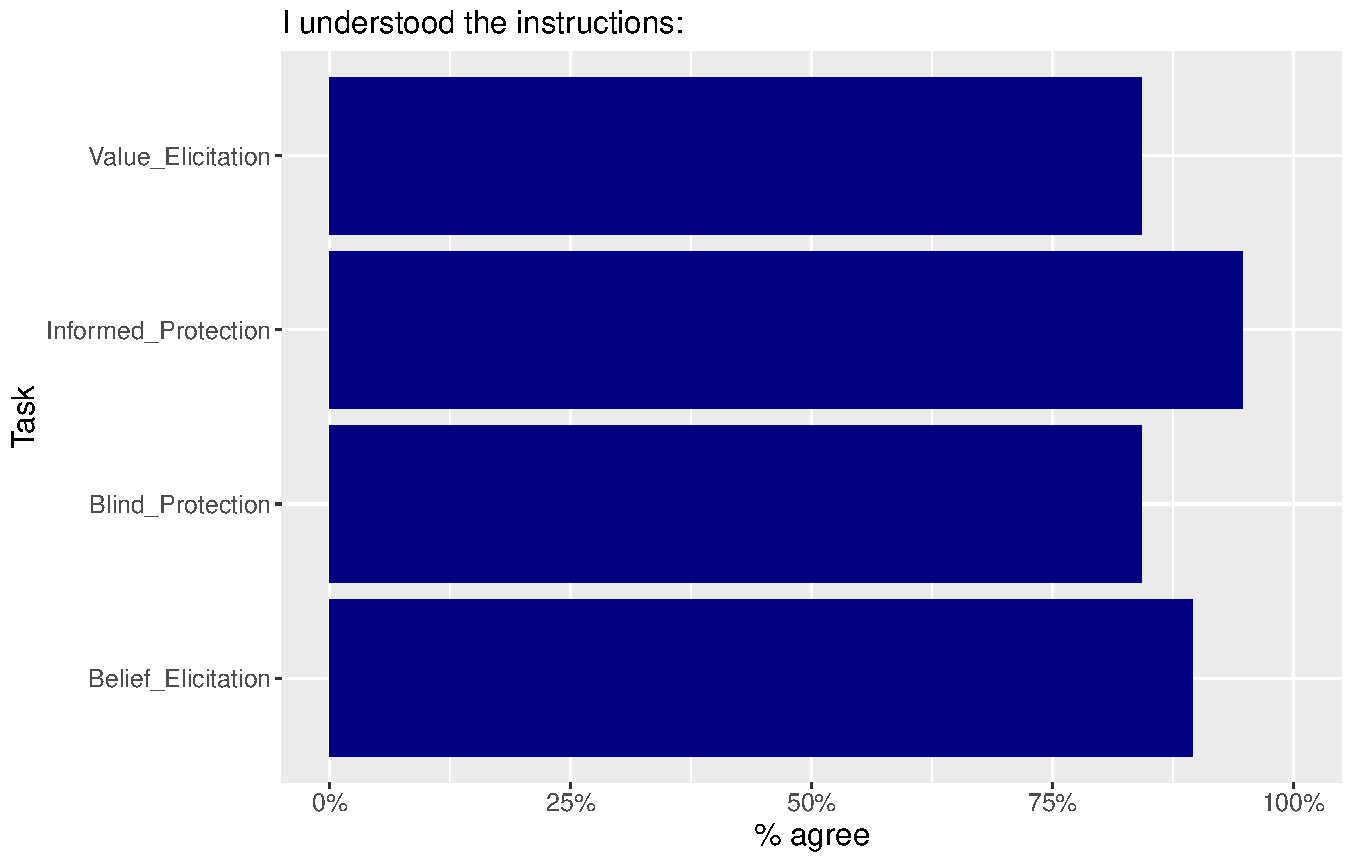
\includegraphics[width=\textwidth]{Graphs/Uplot1.pdf}
\end{subfigure}
~
\begin{subfigure}{0.45\textwidth}
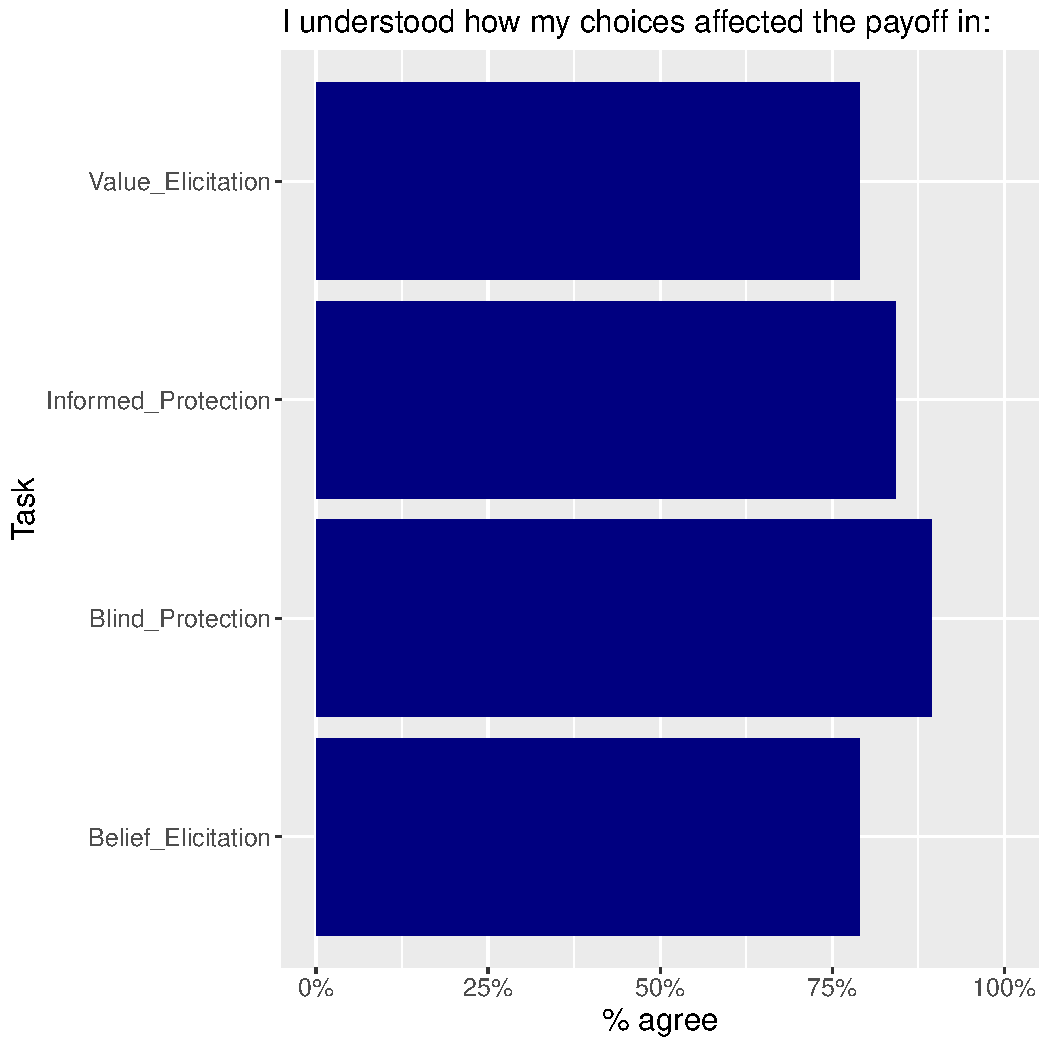
\includegraphics[width=\textwidth]{Graphs/Uplot2.pdf}
\end{subfigure}
\end{figure}
\end{frame}


\begin{frame}
\frametitle{Quiz answers correct}
\begin{itemize}
\item Most respondents make 1-3 mistakes out of 9 questions
\end{itemize}
\begin{figure}[h]
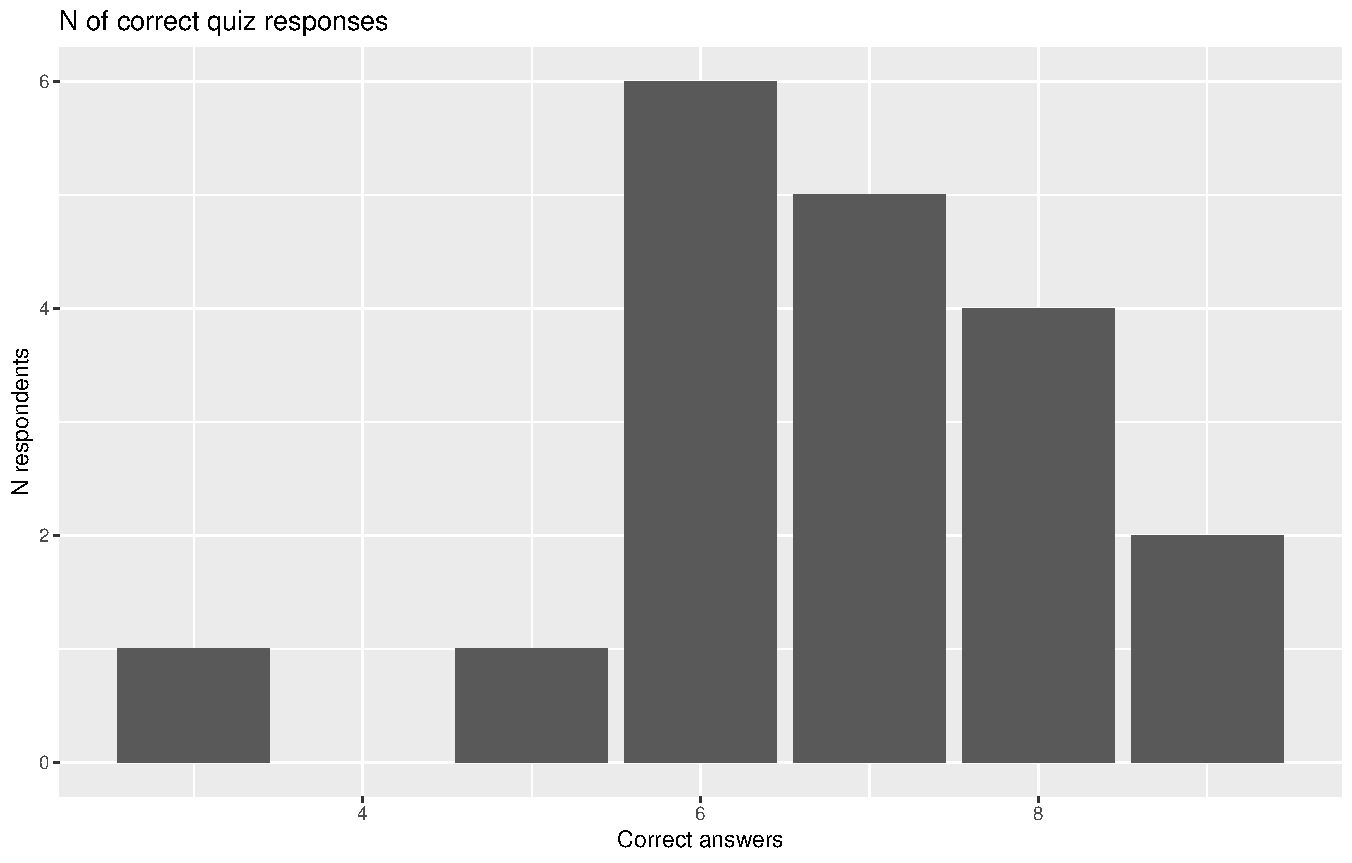
\includegraphics[scale=0.4]{Graphs/COMPRplot.pdf}
\end{figure}
\end{frame}





\begin{frame}
\frametitle{Uninformed Protection}
\begin{itemize}
\item There is more protection when the probability of black ball is higher
\item Noisy
\end{itemize}
\begin{figure}[h]
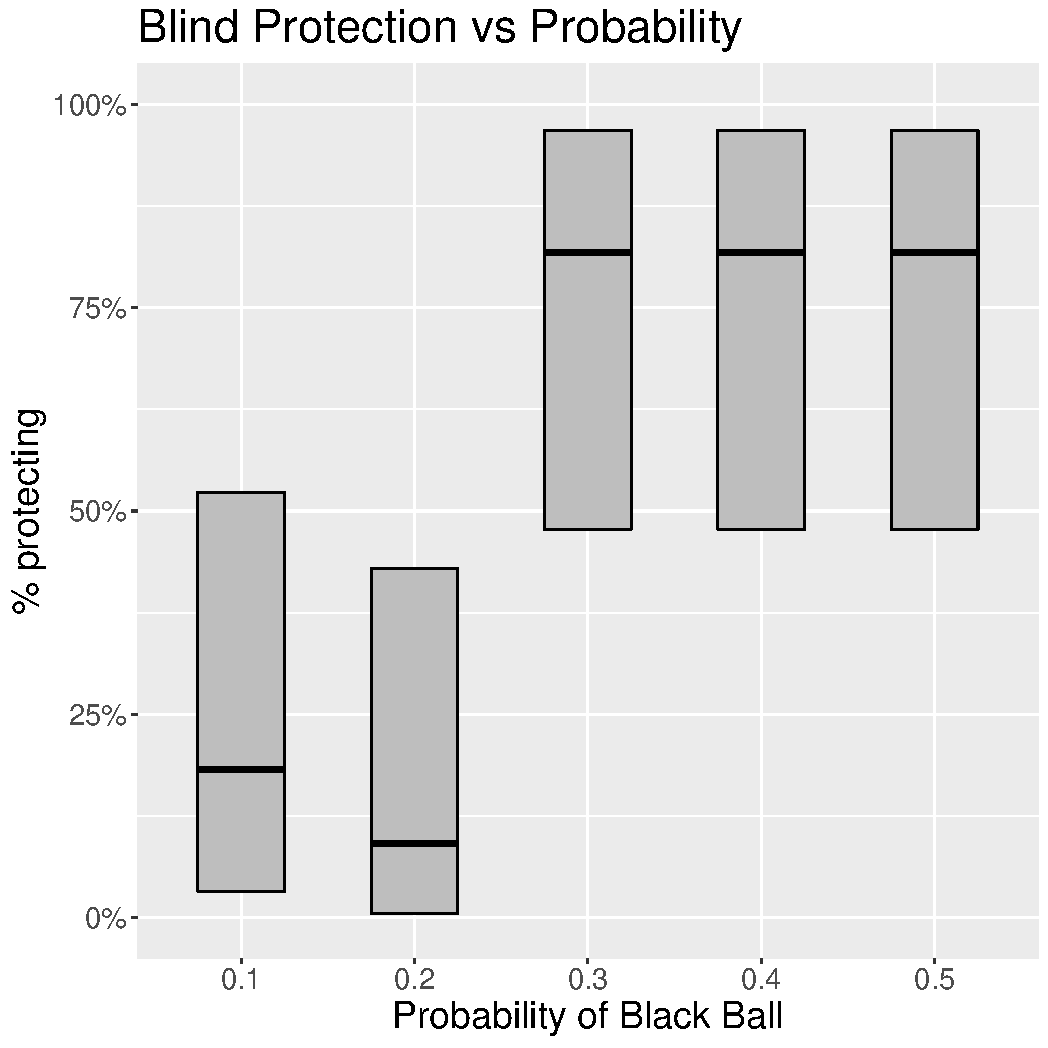
\includegraphics[scale=0.4]{Graphs/BLProt_plot2.pdf}
\end{figure}
\end{frame}




\begin{frame}
\frametitle{Informed Protection}
\begin{itemize}
\item There is more protection when the posterior probability of black ball is higher
\item Even more noisy, but hopefully corrected with larger sample
\item Need to check individual responses (fixed effects)
\end{itemize}
\begin{figure}[h]
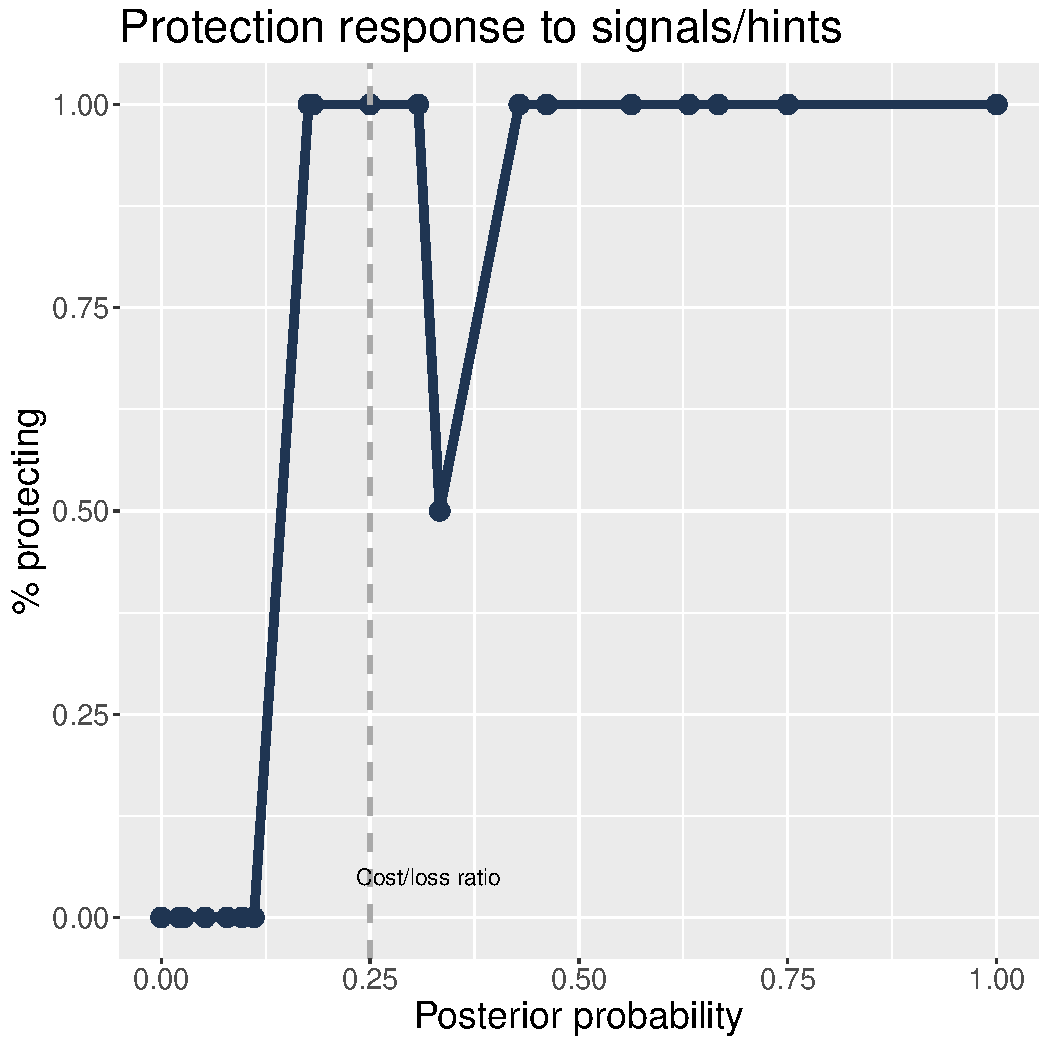
\includegraphics[scale=0.35]{Graphs/IP_plot.pdf}
\end{figure}
\end{frame}
\fi


\begin{frame}
\frametitle{Informed Protection: Correlation}
\footnotesize
\begin{table}[htbp]\centering
\def\sym#1{\ifmmode^{#1}\else\(^{#1}\)\fi}
\caption{Informed Protection}
\begin{tabular}{l*{4}{c}}
\hline\hline
                &\multicolumn{1}{c}{(1)}&\multicolumn{1}{c}{(2)}&\multicolumn{1}{c}{(3)}&\multicolumn{1}{c}{(4)}\\
                &\multicolumn{1}{c}{All}&\multicolumn{1}{c}{All}&\multicolumn{1}{c}{Smart}&\multicolumn{1}{c}{Smart}\\
\hline
Posterior prob. &     .663\sym{***}&     .114         &     .692\sym{***}&     .126         \\
                &    (8.5)         &    (0.9)         &    (9.4)         &    (0.8)         \\
Prior prob.     &                  &     .467\sym{***}&                  &     .519\sym{***}\\
                &                  &    (3.5)         &                  &    (3.1)         \\
Gremlin says Black&                  &     .497\sym{***}&                  &     .506\sym{***}\\
                &                  &    (5.8)         &                  &    (5.0)         \\
Constant        &     .235\sym{***}&    .0872\sym{**} &     .233\sym{***}&    .0678         \\
                &    (7.3)         &    (2.2)         &    (7.7)         &    (1.6)         \\
\hline
Observations    &      300         &      300         &      228         &      228         \\
Adjusted \(R^{2}\)&     0.35         &     0.41         &     0.36         &     0.42         \\
\hline\hline
\multicolumn{5}{l}{\footnotesize \textit{t} statistics in parentheses}\\
\multicolumn{5}{l}{\footnotesize \sym{*} \(p<0.10\), \sym{**} \(p<0.05\), \sym{***} \(p<0.01\)}\\
\end{tabular}
\end{table}

\end{frame}



\begin{frame}
\frametitle{Informed Protection: Determinants}
\footnotesize
\begin{table}[htbp]\centering
\def\sym#1{\ifmmode^{#1}\else\(^{#1}\)\fi}
\caption{Informed Protection: Response to Reported Beliefs}
\begin{tabular}{l*{3}{c}}
\hline\hline
                &\multicolumn{1}{c}{(1)}&\multicolumn{1}{c}{(2)}&\multicolumn{1}{c}{(3)}\\
                &\multicolumn{1}{c}{All}&\multicolumn{1}{c}{All}&\multicolumn{1}{c}{Smart}\\
\hline
Belief          &     .746\sym{***}&     .358\sym{**} &     .462\sym{**} \\
                &    (7.8)         &    (2.4)         &    (2.5)         \\
Posterior prob. &                  &     .424\sym{***}&     .367\sym{**} \\
                &                  &    (3.5)         &    (2.6)         \\
Constant        &     .206\sym{***}&     .189\sym{***}&     .178\sym{***}\\
                &    (5.3)         &    (4.8)         &    (4.6)         \\
\hline
Observations    &      300         &      300         &      228         \\
Adjusted \(R^{2}\)&     0.32         &     0.38         &     0.40         \\
\hline\hline
\multicolumn{4}{l}{\footnotesize \textit{t} statistics in parentheses}\\
\multicolumn{4}{l}{\footnotesize \sym{*} \(p<0.10\), \sym{**} \(p<0.05\), \sym{***} \(p<0.01\)}\\
\end{tabular}
\end{table}

\end{frame}


\begin{frame}
\frametitle{Informed Protection: Do Subject's Beliefs Matter?}
\footnotesize
\begin{table}[htbp]\centering
\def\sym#1{\ifmmode^{#1}\else\(^{#1}\)\fi}
\caption{Informed Protection: Response to Reported Beliefs}
\begin{tabular}{l*{3}{c}}
\hline\hline
                &\multicolumn{1}{c}{(1)}&\multicolumn{1}{c}{(2)}&\multicolumn{1}{c}{(3)}\\
                &\multicolumn{1}{c}{All}&\multicolumn{1}{c}{All}&\multicolumn{1}{c}{Smart}\\
\hline
Belief          &     .746\sym{***}&     .358\sym{**} &     .462\sym{**} \\
                &    (7.8)         &    (2.4)         &    (2.5)         \\
Posterior prob. &                  &     .424\sym{***}&     .367\sym{**} \\
                &                  &    (3.5)         &    (2.6)         \\
Constant        &     .206\sym{***}&     .189\sym{***}&     .178\sym{***}\\
                &    (5.3)         &    (4.8)         &    (4.6)         \\
\hline
Observations    &      300         &      300         &      228         \\
Adjusted \(R^{2}\)&     0.32         &     0.38         &     0.40         \\
\hline\hline
\multicolumn{4}{l}{\footnotesize \textit{t} statistics in parentheses}\\
\multicolumn{4}{l}{\footnotesize \sym{*} \(p<0.10\), \sym{**} \(p<0.05\), \sym{***} \(p<0.01\)}\\
\end{tabular}
\end{table}

\end{frame}



\iffalse
\begin{frame}
\frametitle{Belief Updating}
\begin{itemize}
\item A bit more correlation with actual posterior probabilities!
\item Even more if we exclude everybody scoring less than 7 out of 9 quiz questions
\end{itemize}
\begin{figure}[h]
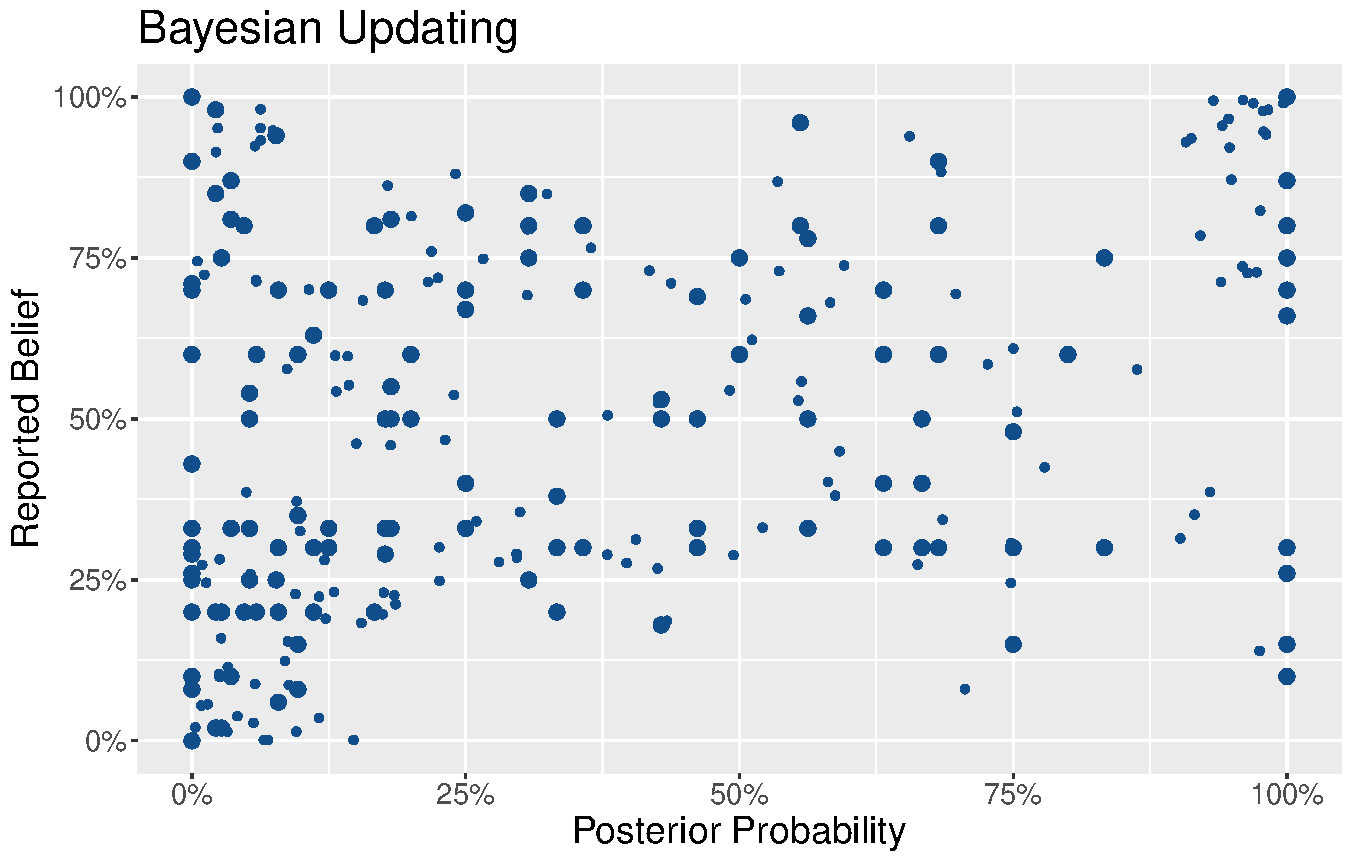
\includegraphics[scale=0.4]{Graphs/UPD_curve2.pdf}
\end{figure}
\end{frame}
\fi

\begin{frame}
\frametitle{Belief Updating: Correlation}
\footnotesize
\begin{table}[htbp]\centering
\def\sym#1{\ifmmode^{#1}\else\(^{#1}\)\fi}
\caption{Belief Elicitation: Belief vs Posterior}
\begin{tabular}{l*{3}{c}}
\hline\hline
                &\multicolumn{1}{c}{(1)}&\multicolumn{1}{c}{(2)}&\multicolumn{1}{c}{(3)}\\
                &\multicolumn{1}{c}{All}&\multicolumn{1}{c}{Not\_honest}&\multicolumn{1}{c}{Good quiz}\\
\hline
Posterior prob. &     .669\sym{***}&     .711\sym{***}&     .523\sym{***}\\
                &   (29.0)         &   (29.1)         &   (15.7)         \\
Constant        &     .151\sym{***}&     .147\sym{***}&     .226\sym{***}\\
                &   (16.2)         &   (14.1)         &   (17.8)         \\
\hline
Observations    &      780         &      636         &      520         \\
Adjusted \(R^{2}\)&     0.57         &     0.61         &     0.39         \\
\hline\hline
\multicolumn{4}{l}{\footnotesize \textit{t} statistics in parentheses}\\
\multicolumn{4}{l}{\footnotesize \sym{*} \(p<0.10\), \sym{**} \(p<0.05\), \sym{***} \(p<0.01\)}\\
\end{tabular}
\end{table}

\end{frame}

\begin{frame}
\frametitle{What Affects Beliefs?}
\footnotesize
\begin{table}[htbp]\centering
\def\sym#1{\ifmmode^{#1}\else\(^{#1}\)\fi}
\caption{Belief Elicitation: Discrepancy}
\begin{tabular}{l*{6}{c}}
\hline\hline
                &\multicolumn{1}{c}{(1)}&\multicolumn{1}{c}{(2)}&\multicolumn{1}{c}{(3)}&\multicolumn{1}{c}{(4)}&\multicolumn{1}{c}{(5)}&\multicolumn{1}{c}{(6)}\\
                &\multicolumn{1}{c}{}&\multicolumn{1}{c}{}&\multicolumn{1}{c}{}&\multicolumn{1}{c}{}&\multicolumn{1}{c}{}&\multicolumn{1}{c}{}\\
\hline
FN rate         &     .016         &     .016         &    -.014         &    -.014         &   -.0562         &   -.0554         \\
                &    (0.1)         &    (0.1)         &    (0.1)         &    (0.1)         &    (0.1)         &    (0.1)         \\
FP rate         &     .919\sym{***}&     .919\sym{***}&     1.07\sym{***}&     1.07\sym{***}&     1.05\sym{***}&     1.05\sym{***}\\
                &    (0.1)         &    (0.1)         &    (0.1)         &    (0.1)         &    (0.1)         &    (0.1)         \\
Good quiz       &                  &                  &    .0469         &    .0673         &                  &                  \\
                &                  &                  &    (0.0)         &    (0.0)         &                  &                  \\
Good quiz $\times$ FN rate&                  &                  &    .0463         &    .0464         &                  &                  \\
                &                  &                  &    (0.1)         &    (0.1)         &                  &                  \\
Good quiz $\times$ FP rate&                  &                  &    -.286\sym{*}  &    -.284\sym{*}  &                  &                  \\
                &                  &                  &    (0.2)         &    (0.2)         &                  &                  \\
Stat. class     &                  &                  &                  &                  &  -.00193         &   -.0127         \\
                &                  &                  &                  &                  &    (0.0)         &    (0.0)         \\
Stat. class $\times$ FN rate&                  &                  &                  &                  &     .127         &     .126         \\
                &                  &                  &                  &                  &    (0.1)         &    (0.1)         \\
Stat. class $\times$ FP rate&                  &                  &                  &                  &    -.229         &    -.226         \\
                &                  &                  &                  &                  &    (0.2)         &    (0.2)         \\
Constant        &    -.076\sym{***}&   -.0656\sym{***}&    -.101\sym{***}&    -.102\sym{***}&   -.0751\sym{***}&   -.0563         \\
                &    (0.0)         &    (0.0)         &    (0.0)         &    (0.0)         &    (0.0)         &    (0.0)         \\
Prior prob dummies &       No         &      Yes         &       No         &      Yes         &       No         &      Yes         \\
\hline
Observations    &      630         &      630         &      630         &      630         &      630         &      630         \\
Adjusted \(R^{2}\)&     0.17         &     0.17         &     0.17         &     0.17         &     0.17         &     0.17         \\
\hline\hline
\multicolumn{7}{l}{\footnotesize Standard errors in parentheses}\\
\multicolumn{7}{l}{\footnotesize \sym{*} \(p<0.10\), \sym{**} \(p<0.05\), \sym{***} \(p<0.01\)}\\
\end{tabular}
\end{table}

\end{frame}

\end{document}
